% Capitolul 8: Seminar - Extensii Moderne
% ARFIMA, Machine Learning, LSTM
% Program de licență, Academia de Studii Economice din București

\documentclass[9pt, aspectratio=169, t]{beamer}

% Ensure content fits on slides
\setbeamersize{text margin left=8mm, text margin right=8mm}

%=============================================================================
% THEME AND STYLE CONFIGURATION
%=============================================================================
\usetheme{Madrid}
\usecolortheme{seahorse}

% IDA-Inspired Color Palette
\definecolor{MainBlue}{RGB}{26, 58, 110}
\definecolor{AccentBlue}{RGB}{42, 82, 140}
\definecolor{IDAred}{RGB}{220, 53, 69}
\definecolor{DarkGray}{RGB}{51, 51, 51}
\definecolor{MediumGray}{RGB}{128, 128, 128}
\definecolor{LightGray}{RGB}{248, 248, 248}
\definecolor{VeryLightGray}{RGB}{235, 235, 235}
\definecolor{Crimson}{RGB}{220, 53, 69}
\definecolor{Forest}{RGB}{46, 125, 50}
\definecolor{Amber}{RGB}{181, 133, 63}
\definecolor{Orange}{RGB}{230, 126, 34}

\setbeamercolor{palette primary}{bg=MainBlue, fg=white}
\setbeamercolor{palette secondary}{bg=MainBlue!85, fg=white}
\setbeamercolor{palette tertiary}{bg=MainBlue!70, fg=white}
\setbeamercolor{structure}{fg=MainBlue}
\setbeamercolor{title}{fg=MainBlue}
\setbeamercolor{frametitle}{fg=MainBlue, bg=white}
\setbeamercolor{block title}{bg=MainBlue, fg=white}
\setbeamercolor{block body}{bg=VeryLightGray, fg=DarkGray}
\setbeamercolor{block title alerted}{bg=Crimson, fg=white}
\setbeamercolor{block body alerted}{bg=Crimson!8, fg=DarkGray}
\setbeamercolor{block title example}{bg=Forest, fg=white}
\setbeamercolor{block body example}{bg=Forest!8, fg=DarkGray}
\setbeamercolor{item}{fg=MainBlue}

\setbeamertemplate{navigation symbols}{}

\setbeamertemplate{footline}{
    \leavevmode%
    \hbox{%
        \begin{beamercolorbox}[wd=.333333\paperwidth,ht=2.5ex,dp=1ex,center]{author in head/foot}%
            \usebeamerfont{author in head/foot}\insertshortauthor
        \end{beamercolorbox}%
        \begin{beamercolorbox}[wd=.333333\paperwidth,ht=2.5ex,dp=1ex,center]{title in head/foot}%
            \usebeamerfont{title in head/foot}\insertshorttitle
        \end{beamercolorbox}%
        \begin{beamercolorbox}[wd=.333333\paperwidth,ht=2.5ex,dp=1ex,right]{date in head/foot}%
            \usebeamerfont{date in head/foot}\insertshortdate{}\hspace*{2em}
            \insertframenumber{} / \inserttotalframenumber\hspace*{2ex}
        \end{beamercolorbox}}%
    \vskip0pt%
}

%=============================================================================
% PACKAGES
%=============================================================================
\usepackage[utf8]{inputenc}
\usepackage[T1]{fontenc}
\usepackage{amsmath, amssymb, amsthm}
\usepackage{mathtools}
\usepackage{bm}
\usepackage{tikz}
\usetikzlibrary{arrows.meta, positioning, shapes, calc}
\usepackage{booktabs}
\usepackage{multirow}
\usepackage{array}
\usepackage{graphicx}
\usepackage{hyperref}
\hypersetup{colorlinks=false, pdfborder={0 0 0}}
\graphicspath{{../logos/}{../charts/}}

%=============================================================================
% CUSTOM COMMANDS
%=============================================================================
\newcommand{\E}{\mathbb{E}}
\newcommand{\Var}{\text{Var}}
\newcommand{\Cov}{\text{Cov}}

%=============================================================================
% TITLE INFORMATION
%=============================================================================
\title[Capitolul 8: Seminar]{Capitolul 8: Seminar --- Extensii Moderne}
\subtitle{Program de licență, Facultatea de Cibernetică, Statistică și Informatică Economică, Academia de Studii Economice din București}
\author[Prof. dr. Daniel Traian Pele]{Prof. dr. Daniel Traian Pele\\[0.2cm]\footnotesize\texttt{danpele@ase.ro}}
\institute{Academia de Studii Economice din București}
\date{An Universitar 2025--2026}

\begin{document}

%=============================================================================
% TITLE SLIDE
%=============================================================================
\begin{frame}[plain]
    \begin{tikzpicture}[remember picture, overlay]
        \fill[IDAred] (current page.north west) rectangle ([yshift=-0.15cm]current page.north east);
        \node[anchor=north west] at ([xshift=0.5cm, yshift=-0.3cm]current page.north west) {
            \href{https://www.ase.ro}{\includegraphics[height=1.1cm]{ase_logo.png}}
        };
        \node[anchor=north] at ([yshift=-0.3cm]current page.north) {
            \href{https://ai4efin.ase.ro}{\includegraphics[height=1.1cm]{ai4efin_logo.png}}
        };
        \node[anchor=north east] at ([xshift=-0.5cm, yshift=-0.3cm]current page.north east) {
            \href{https://www.digital-finance-msca.com}{\includegraphics[height=1.1cm]{msca_logo.png}}
        };
    \end{tikzpicture}
    \vfill
    \begin{center}
        {\Large\textcolor{MediumGray}{Analiza și Prognoza Seriilor de Timp}}\\[0.3cm]
        {\Huge\textbf{\textcolor{MainBlue}{Capitolul 8: Extensii Moderne}}}\\[0.5cm]
        {\Large\textcolor{IDAred}{Seminar}}
    \end{center}
    \vfill

    \begin{tikzpicture}[remember picture, overlay]
        \fill[IDAred] (current page.south west) rectangle ([yshift=0.15cm]current page.south east);
        \node[anchor=south west] at ([xshift=0.5cm, yshift=0.8cm]current page.south west) {
            \href{https://theida.net}{\includegraphics[height=0.9cm]{ida_logo.png}}
        };
        \node[anchor=south] at ([xshift=-3cm, yshift=0.8cm]current page.south) {
            \href{https://blockchain-research-center.com}{\includegraphics[height=0.9cm]{brc_logo.png}}
        };
        \node[anchor=south] at ([yshift=0.8cm]current page.south) {
            \href{https://quantinar.com}{\includegraphics[height=0.9cm]{qr_logo.png}}
        };
        \node[anchor=south] at ([xshift=3cm, yshift=0.8cm]current page.south) {
            \href{https://quantlet.com}{\includegraphics[height=0.9cm]{ql_logo.png}}
        };
        \node[anchor=south east] at ([xshift=-0.5cm, yshift=0.8cm]current page.south east) {
            \href{https://ipe.ro/new}{\includegraphics[height=0.9cm]{acad_logo.png}}
        };
    \end{tikzpicture}
\end{frame}

%=============================================================================
% OUTLINE
%=============================================================================
\begin{frame}{Cuprins Seminar}
    \tableofcontents
\end{frame}

%=============================================================================
% SECTION 1: ARFIMA QUIZ
%=============================================================================
\section{Test: Modele ARFIMA și Memorie Lungă}

\begin{frame}{Test 1: Exponentul Hurst}
    \begin{alertblock}{Întrebare}
        O serie de timp are exponentul Hurst $H = 0.8$. Ce ne indică acest lucru?
    \end{alertblock}

    \vspace{0.3cm}

    \begin{enumerate}[A)]
        \item Seria este un mers aleator pur
        \item Seria are memorie lungă și este persistentă (trend-following)
        \item Seria este anti-persistentă (mean-reverting)
        \item Seria este staționară I(0)
    \end{enumerate}

    \vspace{0.5cm}
    \begin{flushright}\textit{Răspunsul pe slide-ul următor...}\end{flushright}
\end{frame}

\begin{frame}{Test 1: Răspuns}
    \begin{exampleblock}{Răspuns: B -- Memorie lungă și persistență}
        \textbf{Interpretare Exponent Hurst:}
        \begin{itemize}
            \item $H = 0.5$: Mers aleator (fără memorie)
            \item $0.5 < H < 1$: \textbf{Persistență} -- tendința continuă
            \item $0 < H < 0.5$: Anti-persistență -- revenire la medie
        \end{itemize}

        \vspace{0.3cm}
        Cu $H = 0.8 > 0.5$:
        \begin{itemize}
            \item Seria are \textbf{memorie lungă}
            \item Valorile mari tind să fie urmate de valori mari
            \item Autocorrelațiile descresc lent (hiperbolic, nu exponențial)
        \end{itemize}
    \end{exampleblock}
\end{frame}

\begin{frame}{Test 2: Parametrul de Diferențiere Fracționară}
    \begin{alertblock}{Întrebare}
        În modelul ARFIMA(p, d, q), parametrul $d$ poate lua valori:
    \end{alertblock}

    \vspace{0.3cm}

    \begin{enumerate}[A)]
        \item Doar valori întregi (0, 1, 2, ...)
        \item Doar $d = 0$ sau $d = 1$
        \item Orice valoare reală, inclusiv fracționară
        \item Doar valori negative
    \end{enumerate}

    \vspace{0.5cm}
    \begin{flushright}\textit{Răspunsul pe slide-ul următor...}\end{flushright}
\end{frame}

\begin{frame}{Test 2: Răspuns}
    \begin{exampleblock}{Răspuns: C -- Orice valoare reală}
        \textbf{Diferențiere fracționară}: $(1-L)^d$ cu $d \in \mathbb{R}$

        \vspace{0.3cm}
        \textbf{Interpretare valori $d$:}
        \begin{itemize}
            \item $d = 0$: Seria staționară (ARMA)
            \item $0 < d < 0.5$: Memorie lungă, staționară
            \item $d = 0.5$: Granița staționar/nestaționară
            \item $0.5 < d < 1$: Memorie lungă, nestaționară
            \item $d = 1$: Diferențiere completă (ARIMA clasic)
        \end{itemize}

        \vspace{0.2cm}
        \textbf{Relația cu Hurst}: $d = H - 0.5$
    \end{exampleblock}
\end{frame}

\begin{frame}{Test 3: Memoria Lungă în Serii Financiare}
    \begin{alertblock}{Întrebare}
        În ce serie financiară este memoria lungă cel mai frecvent documentată?
    \end{alertblock}

    \vspace{0.3cm}

    \begin{enumerate}[A)]
        \item Prețurile acțiunilor
        \item Randamentele zilnice
        \item Volatilitatea (pătratul randamentelor)
        \item Volumul de tranzacționare
    \end{enumerate}

    \vspace{0.5cm}
    \begin{flushright}\textit{Răspunsul pe slide-ul următor...}\end{flushright}
\end{frame}

\begin{frame}{Test 3: Răspuns}
    \begin{exampleblock}{Răspuns: C -- Volatilitatea}
        \textbf{Fapte stilizate din finanțe:}
        \begin{itemize}
            \item \textbf{Randamentele}: Aproximativ fără memorie ($H \approx 0.5$)
            \item \textbf{Volatilitatea}: Memorie lungă pronunțată ($H \approx 0.7-0.9$)
        \end{itemize}

        \vspace{0.3cm}
        \textbf{De ce?}
        \begin{itemize}
            \item Volatility clustering: perioade agitate urmate de perioade agitate
            \item Persistența șocurilor în varianță
            \item FIGARCH: modelează explicit memoria lungă în volatilitate
        \end{itemize}

        \vspace{0.2cm}
        {\footnotesize Acest fapt stilizat este baza modelelor FIGARCH și HAR-RV.}
    \end{exampleblock}
\end{frame}

%=============================================================================
% SECTION 2: MACHINE LEARNING QUIZ
%=============================================================================
\section{Test: Machine Learning pentru Serii de Timp}

\begin{frame}{Test 4: Feature Engineering}
    \begin{alertblock}{Întrebare}
        Pentru a aplica Random Forest pe serii de timp, trebuie să creăm:
    \end{alertblock}

    \vspace{0.3cm}

    \begin{enumerate}[A)]
        \item Variabile dummy pentru fiecare observație
        \item Caracteristici lag și statistici rolling
        \item Transformări Fourier ale seriei
        \item Numai prima diferență a seriei
    \end{enumerate}

    \vspace{0.5cm}
    \begin{flushright}\textit{Răspunsul pe slide-ul următor...}\end{flushright}
\end{frame}

\begin{frame}{Test 4: Răspuns}
    \begin{exampleblock}{Răspuns: B -- Caracteristici lag și statistici rolling}
        \textbf{Feature Engineering pentru Serii de Timp:}

        \vspace{0.2cm}
        \begin{itemize}
            \item \textbf{Lag features}: $y_{t-1}, y_{t-2}, \ldots, y_{t-k}$
            \item \textbf{Rolling statistics}:
                \begin{itemize}
                    \item Media mobilă: $\bar{y}_{t,w}$
                    \item Deviația standard mobilă: $\sigma_{t,w}$
                    \item Min/Max pe fereastră
                \end{itemize}
            \item \textbf{Caracteristici calendaristice}: ziua săptămânii, luna, etc.
        \end{itemize}

        \vspace{0.2cm}
        \textbf{Important}: Transformă problema de prognoză în problemă de regresie supervizată!
    \end{exampleblock}
\end{frame}

\begin{frame}{Test 5: Validarea Încrucișată pentru Serii de Timp}
    \begin{alertblock}{Întrebare}
        De ce NU putem folosi k-fold cross-validation standard pentru serii de timp?
    \end{alertblock}

    \vspace{0.3cm}

    \begin{enumerate}[A)]
        \item Este prea lent pentru serii lungi
        \item Încalcă ordinea temporală și cauzează data leakage
        \item Funcționează doar pentru clasificare
        \item Necesită prea multe date
    \end{enumerate}

    \vspace{0.5cm}
    \begin{flushright}\textit{Răspunsul pe slide-ul următor...}\end{flushright}
\end{frame}

\begin{frame}{Test 5: Răspuns}
    \begin{exampleblock}{Răspuns: B -- Încalcă ordinea temporală}
        \textbf{Problema cu k-fold standard:}
        \begin{itemize}
            \item Amestecă observațiile temporal
            \item Antrenează pe date din viitor, testează pe trecut
            \item \textbf{Data leakage} $\Rightarrow$ performanță supraestimată
        \end{itemize}

        \vspace{0.3cm}
        \textbf{Soluția: Time Series Split (Walk-Forward)}
        \begin{center}
        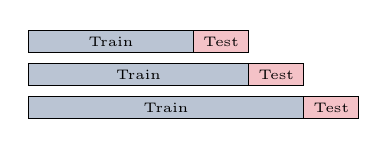
\begin{tikzpicture}[scale=0.7]
            \draw[fill=MainBlue!30] (0,0) rectangle (3,0.4) node[midway] {\tiny Train};
            \draw[fill=Crimson!30] (3,0) rectangle (4,0.4) node[midway] {\tiny Test};
            \draw[fill=MainBlue!30] (0,-0.6) rectangle (4,-0.2) node[midway] {\tiny Train};
            \draw[fill=Crimson!30] (4,-0.6) rectangle (5,-0.2) node[midway] {\tiny Test};
            \draw[fill=MainBlue!30] (0,-1.2) rectangle (5,-0.8) node[midway] {\tiny Train};
            \draw[fill=Crimson!30] (5,-1.2) rectangle (6,-0.8) node[midway] {\tiny Test};
        \end{tikzpicture}
        \end{center}
    \end{exampleblock}
\end{frame}

\begin{frame}{Test 6: Importanța Variabilelor în Random Forest}
    \begin{alertblock}{Întrebare}
        Importanța variabilelor în Random Forest pentru serii de timp ne ajută să:
    \end{alertblock}

    \vspace{0.3cm}

    \begin{enumerate}[A)]
        \item Să eliminăm toate variabilele cu importanță mică
        \item Să identificăm care lag-uri și caracteristici sunt cele mai predictive
        \item Să determinăm cauzalitatea Granger
        \item Să calculăm intervalele de încredere
    \end{enumerate}

    \vspace{0.5cm}
    \begin{flushright}\textit{Răspunsul pe slide-ul următor...}\end{flushright}
\end{frame}

\begin{frame}{Test 6: Răspuns}
    \begin{exampleblock}{Răspuns: B -- Identifică caracteristicile predictive}
        \textbf{Utilizări ale importanței variabilelor:}
        \begin{itemize}
            \item Înțelegerea structurii temporale
            \item Selectarea numărului optim de lag-uri
            \item Identificarea factorilor relevanți
        \end{itemize}

        \vspace{0.3cm}
        \textbf{Atenție:}
        \begin{itemize}
            \item Importanța NU implică cauzalitate
            \item Variabilele corelate pot împărtăși importanța
            \item Folosiți pentru interpretare, nu pentru inferență cauzală
        \end{itemize}
    \end{exampleblock}
\end{frame}

%=============================================================================
% SECTION 3: LSTM QUIZ
%=============================================================================
\section{Test: Rețele LSTM}

\begin{frame}{Test 7: Avantajul LSTM}
    \begin{alertblock}{Întrebare}
        Care este principalul avantaj al LSTM față de RNN simple?
    \end{alertblock}

    \vspace{0.3cm}

    \begin{enumerate}[A)]
        \item Este mai rapidă la antrenare
        \item Rezolvă problema gradienților care dispar/explodează
        \item Necesită mai puține date
        \item Este mai ușor de interpretat
    \end{enumerate}

    \vspace{0.5cm}
    \begin{flushright}\textit{Răspunsul pe slide-ul următor...}\end{flushright}
\end{frame}

\begin{frame}{Test 7: Răspuns}
    \begin{exampleblock}{Răspuns: B -- Rezolvă problema gradienților}
        \textbf{Problema RNN Simple:}
        \begin{itemize}
            \item Gradienții scad exponențial cu lungimea secvenței
            \item Nu pot învăța dependențe pe termen lung
        \end{itemize}

        \vspace{0.3cm}
        \textbf{Soluția LSTM:}
        \begin{itemize}
            \item \textbf{Cell state}: Autostradă pentru flux de informație
            \item \textbf{Forget gate}: Decide ce să uite
            \item \textbf{Input gate}: Decide ce să rețină
            \item \textbf{Output gate}: Decide ce să producă
        \end{itemize}

        \vspace{0.2cm}
        Gradienții pot „curge" prin cell state fără degradare!
    \end{exampleblock}
\end{frame}

\begin{frame}{Test 8: Pregătirea Datelor pentru LSTM}
    \begin{alertblock}{Întrebare}
        Înainte de antrenarea LSTM, datele trebuie:
    \end{alertblock}

    \vspace{0.3cm}

    \begin{enumerate}[A)]
        \item Transformate logaritmic
        \item Normalizate/standardizate la intervalul [0,1] sau [-1,1]
        \item Diferențiate de ordinul 2
        \item Convertite la numere întregi
    \end{enumerate}

    \vspace{0.5cm}
    \begin{flushright}\textit{Răspunsul pe slide-ul următor...}\end{flushright}
\end{frame}

\begin{frame}{Test 8: Răspuns}
    \begin{exampleblock}{Răspuns: B -- Normalizate/standardizate}
        \textbf{De ce normalizare?}
        \begin{itemize}
            \item Funcțiile de activare (sigmoid, tanh) funcționează în intervale limitate
            \item Convergență mai rapidă
            \item Stabilitate numerică
        \end{itemize}

        \vspace{0.3cm}
        \textbf{Metode comune:}
        \begin{itemize}
            \item \textbf{Min-Max}: $x' = \frac{x - x_{min}}{x_{max} - x_{min}}$ $\succ$ [0, 1]
            \item \textbf{Standard}: $x' = \frac{x - \mu}{\sigma}$ $\succ$ media 0, std 1
        \end{itemize}

        \vspace{0.2cm}
        \textbf{Important}: Fit pe train, transform pe train+test!
    \end{exampleblock}
\end{frame}

\begin{frame}{Test 9: Hiperparametri LSTM}
    \begin{alertblock}{Întrebare}
        Care NU este un hiperparametru tipic pentru LSTM?
    \end{alertblock}

    \vspace{0.3cm}

    \begin{enumerate}[A)]
        \item Numărul de unități (neuroni) pe strat
        \item Lungimea secvenței de intrare
        \item Learning rate
        \item Parametrul de diferențiere $d$
    \end{enumerate}

    \vspace{0.5cm}
    \begin{flushright}\textit{Răspunsul pe slide-ul următor...}\end{flushright}
\end{frame}

\begin{frame}{Test 9: Răspuns}
    \begin{exampleblock}{Răspuns: D -- Parametrul $d$}
        $d$ este specific modelelor ARFIMA, nu LSTM!

        \vspace{0.3cm}
        \textbf{Hiperparametri LSTM:}
        \begin{itemize}
            \item \textbf{Arhitectură}: nr. straturi, unități/strat
            \item \textbf{Secvență}: lungime lookback
            \item \textbf{Training}: learning rate, batch size, epochs
            \item \textbf{Regularizare}: dropout, early stopping
        \end{itemize}

        \vspace{0.2cm}
        \textbf{Tuning}: Grid search sau Bayesian optimization cu time series CV
    \end{exampleblock}
\end{frame}

%=============================================================================
% SECTION 4: PRACTICAL PROBLEMS
%=============================================================================
\section{Probleme Practice}

\begin{frame}{Problemă 1: Estimarea Exponentului Hurst}
    \begin{block}{Enunț}
        Fie seria zilnică de randamente Bitcoin. Estimați exponentul Hurst folosind metoda R/S și interpretați rezultatul.
    \end{block}

    \vspace{0.3cm}
    \textbf{Pași de rezolvare:}
    \begin{enumerate}
        \item Calculați media pe subintervale de diferite lungimi $n$
        \item Pentru fiecare $n$: calculați Range($R$) și Std($S$)
        \item Raportul $R/S$ crește ca $n^H$
        \item Fit regresie: $\log(R/S) = H \cdot \log(n) + c$
    \end{enumerate}

    \vspace{0.2cm}
    \textbf{Cod Python}: \texttt{nolds.hurst\_rs(returns)}
\end{frame}

\begin{frame}{Problemă 1: Soluție și Interpretare}
    \begin{exampleblock}{Rezultat Tipic pentru Bitcoin}
        \begin{itemize}
            \item Randamente: $H \approx 0.45-0.55$ (aproape mers aleator)
            \item Volatilitate (|returns|): $H \approx 0.75-0.85$ (memorie lungă!)
        \end{itemize}
    \end{exampleblock}

    \vspace{0.3cm}
    \textbf{Interpretare:}
    \begin{itemize}
        \item Randamentele sunt greu de prognozat (EMH aproximativ validă)
        \item Volatilitatea este predictibilă pe termen lung
        \item Implicații pentru managementul riscului și VaR
    \end{itemize}

    \vspace{0.2cm}
    \textbf{Aplicație}: Modelele FIGARCH pot fi superioare GARCH standard
\end{frame}

\begin{frame}{Problemă 2: Random Forest pentru Prognoză}
    \begin{block}{Enunț}
        Construiți un model Random Forest pentru prognoza prețului Bitcoin la orizontul de 1 zi. Evaluați folosind TimeSeriesSplit.
    \end{block}

    \vspace{0.3cm}
    \textbf{Pipeline:}
    \begin{enumerate}
        \item \textbf{Feature engineering}:
            \begin{itemize}
                \item Lag-uri: $y_{t-1}, y_{t-2}, \ldots, y_{t-7}$
                \item Rolling mean/std: 7, 14, 30 zile
            \end{itemize}
        \item \textbf{Train/Test split}: TimeSeriesSplit(n\_splits=5)
        \item \textbf{Model}: RandomForestRegressor(n\_estimators=100)
        \item \textbf{Evaluare}: RMSE, MAE, Direction Accuracy
    \end{enumerate}
\end{frame}

\begin{frame}{Problemă 2: Cod și Rezultate}
    \begin{exampleblock}{Cod Python}
        {\footnotesize
        \texttt{from sklearn.ensemble import RandomForestRegressor}\\
        \texttt{from sklearn.model\_selection import TimeSeriesSplit}\\[0.2cm]
        \texttt{tscv = TimeSeriesSplit(n\_splits=5)}\\
        \texttt{rf = RandomForestRegressor(n\_estimators=100)}\\[0.2cm]
        \texttt{for train\_idx, test\_idx in tscv.split(X):}\\
        \texttt{~~~~rf.fit(X[train\_idx], y[train\_idx])}\\
        \texttt{~~~~pred = rf.predict(X[test\_idx])}
        }
    \end{exampleblock}

    \vspace{0.2cm}
    \textbf{Rezultate tipice}:
    \begin{itemize}
        \item Direction accuracy: 52-55\% (puțin peste random)
        \item Feature importance: lag-1 și rolling\_std domină
    \end{itemize}
\end{frame}

\begin{frame}{Problemă 3: LSTM pentru Serii de Timp}
    \begin{block}{Enunț}
        Implementați un model LSTM simplu pentru prognoza Bitcoin. Comparați cu Random Forest.
    \end{block}

    \vspace{0.3cm}
    \textbf{Arhitectură LSTM simplă:}
    \begin{enumerate}
        \item Input: secvențe de 30 de zile
        \item LSTM layer: 50 unități
        \item Dense output: 1 neuron (prognoza)
        \item Loss: MSE, Optimizer: Adam
    \end{enumerate}

    \vspace{0.2cm}
    \textbf{Pași importanți}:
    \begin{itemize}
        \item Normalizare MinMaxScaler
        \item Reshape la [samples, timesteps, features]
        \item Early stopping pentru a evita supraajustare
    \end{itemize}
\end{frame}

\begin{frame}{Problemă 3: Cod LSTM}
    \begin{exampleblock}{Cod Keras/TensorFlow}
        {\footnotesize
        \texttt{from tensorflow.keras.models import Sequential}\\
        \texttt{from tensorflow.keras.layers import LSTM, Dense}\\[0.2cm]
        \texttt{model = Sequential([}\\
        \texttt{~~~~LSTM(50, input\_shape=(30, 1)),}\\
        \texttt{~~~~Dense(1)}\\
        \texttt{])}\\[0.2cm]
        \texttt{model.compile(optimizer='adam', loss='mse')}\\
        \texttt{model.fit(X\_train, y\_train, epochs=50,}\\
        \texttt{~~~~~~~~~~validation\_split=0.1, verbose=0)}
        }
    \end{exampleblock}

    \vspace{0.2cm}
    \textbf{Comparație tipică RF vs LSTM}:
    \begin{itemize}
        \item RMSE similar (LSTM ușor mai bun pe date netede)
        \item RF: mai rapid, mai interpretabil
        \item LSTM: captează mai bine pattern-uri complexe
    \end{itemize}
\end{frame}

%=============================================================================
% SECTION 5: SUMMARY
%=============================================================================
\section{Recapitulare}

\begin{frame}{Rezumat: Când să Folosim Fiecare Metodă}
    \begin{block}{ARFIMA}
        \begin{itemize}
            \item Serii cu memorie lungă (volatilitate, hidrologie)
            \item Când $0 < d < 0.5$ este teoretic justificat
            \item Interpretabilitate statistică importantă
        \end{itemize}
    \end{block}

    \begin{block}{Random Forest}
        \begin{itemize}
            \item Relații neliniare între caracteristici
            \item Feature importance pentru înțelegere
            \item Date structurate, nu foarte lungi
        \end{itemize}
    \end{block}

    \begin{block}{LSTM}
        \begin{itemize}
            \item Secvențe lungi cu dependențe complexe
            \item Date suficiente pentru deep learning
            \item Pattern-uri dificil de capturat cu metode clasice
        \end{itemize}
    \end{block}
\end{frame}

\begin{frame}{Formule Cheie}
    \begin{block}{ARFIMA și Memorie Lungă}
        \begin{itemize}
            \item Diferențiere fracționară: $(1-L)^d y_t = \varepsilon_t$
            \item Exponent Hurst: $d = H - 0.5$
            \item ACF pentru memorie lungă: $\rho(k) \sim k^{2d-1}$ (descreștere lentă)
        \end{itemize}
    \end{block}

    \begin{block}{Machine Learning}
        \begin{itemize}
            \item Feature lag: $X_t = [y_{t-1}, y_{t-2}, \ldots, y_{t-k}]$
            \item RMSE: $\sqrt{\frac{1}{n}\sum(y_i - \hat{y}_i)^2}$
            \item Direction Accuracy: $\frac{1}{n}\sum \mathbf{1}[\text{sign}(\Delta y) = \text{sign}(\Delta \hat{y})]$
        \end{itemize}
    \end{block}

    \begin{block}{LSTM}
        \begin{itemize}
            \item Forget gate: $f_t = \sigma(W_f \cdot [h_{t-1}, x_t] + b_f)$
            \item Cell update: $C_t = f_t * C_{t-1} + i_t * \tilde{C}_t$
        \end{itemize}
    \end{block}
\end{frame}

%=============================================================================
% THANK YOU SLIDE
%=============================================================================
\begin{frame}[plain]
    \begin{tikzpicture}[remember picture, overlay]
        \fill[IDAred] (current page.north west) rectangle ([yshift=-0.15cm]current page.north east);
    \end{tikzpicture}
    \vfill
    \begin{center}
        {\Huge\textbf{\textcolor{MainBlue}{Vă mulțumesc!}}}\\[1cm]
        {\Large Întrebări?}\\[0.5cm]
        {\large\texttt{danpele@ase.ro}}
    \end{center}
    \vfill
    \begin{tikzpicture}[remember picture, overlay]
        \fill[IDAred] (current page.south west) rectangle ([yshift=0.15cm]current page.south east);
    \end{tikzpicture}
\end{frame}

\end{document}
